%%=============================================================================
%% Methodologie
%%=============================================================================

\chapter{\IfLanguageName{dutch}{Methodologie}{Methodology}}%
\label{ch:methodologie}

%% TODO: In dit hoofstuk geef je een korte toelichting over hoe je te werk bent
%% gegaan. Verdeel je onderzoek in grote fasen, en licht in elke fase toe wat
%% de doelstelling was, welke deliverables daar uit gekomen zijn, en welke
%% onderzoeksmethoden je daarbij toegepast hebt. Verantwoord waarom je
%% op deze manier te werk gegaan bent.
%% 
%% Voorbeelden van zulke fasen zijn: literatuurstudie, opstellen van een
%% requirements-analyse, opstellen long-list (bij vergelijkende studie),
%% selectie van geschikte tools (bij vergelijkende studie, "short-list"),
%% opzetten testopstelling/PoC, uitvoeren testen en verzamelen
%% van resultaten, analyse van resultaten, ...
%%
%% !!!!! LET OP !!!!!
%%
%% Het is uitdrukkelijk NIET de bedoeling dat je het grootste deel van de corpus
%% van je bachelorproef in dit hoofstuk verwerkt! Dit hoofdstuk is eerder een
%% kort overzicht van je plan van aanpak.
%%
%% Maak voor elke fase (behalve het literatuuronderzoek) een NIEUW HOOFDSTUK aan
%% en geef het een gepaste titel.
%% \lipsum[21-25]

Het onderzoek naar de ontwikkeling en integratie van een Netskope-gebaseerde Data Leakage Prevention (DLP)-oplossing binnen 
de bedrijfsomgeving van Evolane. De onderzoeksmethode is een combinatie van een literatuurstudie en een praktische Proof of Concept (PoC).

\section{Literatuurstudie}%

Het onderzoek begint met een uitgebreide literatuurstudie naar bestaande DLP-oplossingen, Netskope's Secure Service Edge (\gls{sse}) platform en de relevante Belgische en Europese wetgevingen. 
Hierbij wordt gebruik gemaakt van academische artikelen, technische documentatie en juridische bronnen om een basis te leggen. 
Voor de literatuurstudie is ongeveer twee weken voorzien, waarin de focus ligt op het verder verzamelen en verwerken van recente bronnen
over DLP-technologie, juridische eisen (\gls{avg}, \gls{pcidss}, \gls{nis2}) en Netskope's DLP-oplossing.

\section{Analyse en planning}%

Na de literatuurstudie volgt de selectie van specifieke datasets, zoals persoonlijk identificeerbare informatie (\gls{pii}) en betalingsgegevens (\gls{pci}), voor testen binnen de PoC.
Een voorbeeld hiervan zijn de synthetische e-maildatasets van \textcite{Whelan2014}. 
Deze datasets bevatten in totaal 4796 e-mails, waarvan 4010 geen \gls{pii} bevatten en 786 e-mails dit wel hebben, 
waaronder adressen, creditcardnummers en namen. 
De opgestelde testscenario's sluiten aan bij de bedrijfsprocessen van Evolane, zoals e-mailverkeer en bestandsoverdrachten naar cloudservices. 
Naast deze scenario's richt de analyse zich ook op de workflow van eindgebruikers, met als doel False Positives te beperken en de de workflow van de eindgebruikers niet te verstoren.
Deze fase begint al deels tijdens de literatuurstudie en duurt ongeveer drie weken.

\section{Risicoanalyse}%

Een belangrijk onderdeel van dit onderzoek is het uitvoeren van een risicoanalyse, waarbij mogelijke technische, juridische en organisatorische risico's worden geïdentificeerd en beoordeeld. 
Technische risico's kunnen bijvoorbeeld bestaan uit het niet volledig detecteren van gevoelige gegevens of prestatieproblemen van het DLP-systeem. 
Juridische risico's hebben te maken met het niet naleven van de \gls{avg}-vereisten of andere relevante wetgeving. 
Organisatorische risico's omvatten mogelijke weerstand van medewerkers tegen nie\-uwe beveiligingsmaatregelen of een gebrek aan training, 
wat de effectiviteit van de DLP-oplossing kan verminderen. 
Voor elk vastgesteld risico worden geschikte maatregelen genomen om de gevolgen te beperken. 
Deze fase duurt ongeveer twee weken, overlappend met Analyse en Planning. Op het vlak van expertise zal hierbij de co-promotor van Evolane betrokken worden. 

\subsection{Technische risico's}

Technische risico's zijn gerelateerd aan de operationele elementen van de DLP-oplossing en de technische infrastructuur van Evolane.
Een van de belangrijkste technische risico's is de onvolledige detectie van confidentiële gegevens. 
Het DLP-systeem kan mogelijk niet alle vormen van \gls{pii} en \gls{pci} detecteren, vooral als er nieuwe of onbekende datatypes worden gebruikt.
Daarnaast kan de implementatie van Netskope leiden tot prestatieproblemen, zoals vertragingen in netwerkverkeer of een verhoogd gebruik van systeemresources.
Integratieproblemen vormen een ander potentieel risico, aangezien het DLP-systeem moet werken met bestaande IT-infrastructuren.
Onverwachte compatibiliteitsproblemen kunnen de implementatie vertragen. Vervolgens kunnen verdere beveiligingslekken ontstaan 
door onvoldoende configuratie of zwakke punten in het DLP-systeem, waardoor confidentiële data alsnog kan worden gelekt.
Om deze technische risico's te mitigeren, zullen uitgebreide tests worden uitgevoerd om de detectienauwkeurigheid van het DLP-systeem te waarborgen.
Daarnaast zullen systeemprestaties worden gemonitord tijdens de implementatie en indien nodig optimalisaties worden doorgevoerd om prestatieproblemen te minimaliseren.
Tenslotte zal een plan worden opgesteld hoe het DLP-systeem veilig geüpdatet kan worden om potentiële kwetsbaarheden te vermijden.

\subsection{Juridische risico's}

Juridische risico's hebben betrekking op de naleving van wet- en regelgeving, zoals de Algemene Verordening Gegevensbescherming (\gls{avg}) en de NIS2-richtlijn.
Onvoldoende naleving van deze wetten en richtlijnen (waaronder \gls{avg}, \gls{pci} DSS, ISO 27001, NIS2, Schrems II,..) kan leiden tot juridische sancties. 
Een belangrijk juridisch risico betreft onjuiste Data Processing Agreements (\gls{dpa}) met dataverwerkers. 
Verkeerde of ontbrekende overeenkomsten met dataverwerkers kunnen juridische complicaties veroorzaken. 
Daarnaast kan het niet correct toepassen van dataminimalisatieprincipes of het verwerken van data voor andere doeleinden dan waarvoor ze zijn verzameld, 
ook leiden tot juridische gevolgen. 
Om deze juridische risico's te beperken, stellen betrokken partijen zorgvuldig \gls{dpa}'s op en voeren zij regelmatige herzieningen uit.

\subsection{Organisatorische risico's}

Organisatorische risico's hebben betrekking op de interne processen en procedures van Evolane en de acceptatie van de DLP-oplossing door medewerkers. 
Weerstand van medewerkers kan een belangrijk organisatorisch risico vormen, aangezien medewerkers mogelijk niet openstaan voor nieuwe beveiligingsmaatregelen. 
Een gebrek aan training kan bovendien leiden tot misbruik of onjuist gebruik van het DLP-systeem, wat de effectiviteit ervan zal verminderen. 
Om dan tenslotte deze organisatorische risico's te mitigeren, zullen workshops en informatiesessies worden georganiseerd om medewerkers te betrekken en het belang van de DLP-oplossing te benadrukken. 
Door medewerkers actief te betrekken en voldoende training te bieden, wordt het gebruik van de DLP-oplossing vergroot en wordt de effectiviteit ervan versterkt.

\section{Proof of Concept}%

De PoC wordt opgezet in een interne testomgeving binnen het bedrijf, waarbij een Netskope-licentie wordt gebruikt om de DLP-service in te stellen. 
Deze omgeving zal verschillende datatypes bevatten (data-in-use, data-in-motion, data-at-rest), 
waarbij zowel vertrouwelijke als niet\--vertr\-ouwelijke bestanden worden gebruikt om te testen of de DLP-service alle vertrouwelijke data effectief kan identificeren en verdere verwerking kan blokkeren. 
De data bestaat voornamelijk uit persoonlijk identificeerbare informatie (\gls{pii}) en betalingsgegevens (\gls{pci}), die volgens de geldende wet- en regelgeving (zoals \gls{avg}, \gls{pci} DSS, ISO 27001, NIS2, Schrems II, enz.) beschermd moeten worden. 
Gebruikers met verschillende rechten zullen data doorsturen en verwerken binnen de testomgeving. 
De duur van de PoC is afhankelijk van de complexiteit van de testscenario's en de detectie van gevoelige gegevens, 
maar wordt geschat op 5 tot 6 weken. 
Na ongeveer 5 weken zou een eerste evaluatie van de effectiviteit van de DLP-oplossing mogelijk moeten zijn, 
en kan deze aan de eindgebruikers van Evolane worden gepresenteerd. 
Voor de technische uitvoering is expertise nodig in de configuratie van Netskope (bijvoorbeeld het instellen van detectie- en preventieregels met regex-patronen), 
evenals basiskennis van de netwerkinfrastructuur van de testomgeving om de dataflows goed na te bootsen.

\section{Gebruikerstests en feedback}%

Na de initiële implementatie van de PoC worden gebruikers van Evolane betrokken bij het testen van de DLP-oplossing. 
Dit gebeurt, samen met mijn co-promotor, door middel van workshops en praktische tests waarbij eindgebruikers realistische scenario's simuleren waarin gevoelige data verwerkt en verplaatst wordt. 
De feedback van deze gebruikers is essentieel om inzicht te krijgen in de gebruiksvriendelijkheid en de invloed van de DLP-regelsets op de dagelijkse taken. 

\section{Evaluatie en meetbare criteria}%

De effectiviteit van de geïmplementeerde DLP-oplossing wordt geëvalueerd aan de hand van vooraf gedefinieerde Key Performance Indicators (\gls{kpi}'s). 
Deze \gls{kpi}'s dienen als indicator om te beoordelen in hoeverre de DLP-oplossing voldoet aan de gestelde vereisten en doelstellingen.
Detectienauwkeurigheid meet het percentage correct geïdentificeerde confidentiële gegevens binnen de totale dataset, 
wat aangeeft hoe effectief de DLP-oplossing is in het herkennen van \gls{pii} en \gls{pci}. 
Het aantal false positives geeft aan hoeveel gegevens onterecht zijn geblokkeerd of gemarkeerd, 
wat inzicht geeft in de nauwkeurigheid van de detectiemethoden en helpt bij het finetunen van de regelsets. 
Dit zal in een Confusion Matrix worden weergegeven \autocite{Microsoftn.d.}.
Systeemimpact zal het effect van de DLP-implementatie op de algehele systeemprestaties beoordelen, zoals CPU- en 
geheugenverbruik, zodat de oplossing geen significante vertragingen of resource-uitputting zou veroorzaken.

\section{Documentatie van resultaten}%

Alle bevindingen en conclusies worden grondig gedocumenteerd. 
In ongeveer twee weken tijd worden handleidingen, een schriftelijk evaluatierapport en het finale concept-bachelorproef geschreven.

\section{Planning}%
\label{sec:planning}

De planning van het onderzoek, weergegeven in figuur \ref{fig:gantBP}, is vastgelegd in een Gantt-diagram. De planning is opgesteld van 17 februari 2025 tot 24 mei 2025, met de laatste twee weken specifiek gereserveerd voor documentatie.

\begin{figure}
  \centering
  % \includegraphics[width=.2\textwidth]
  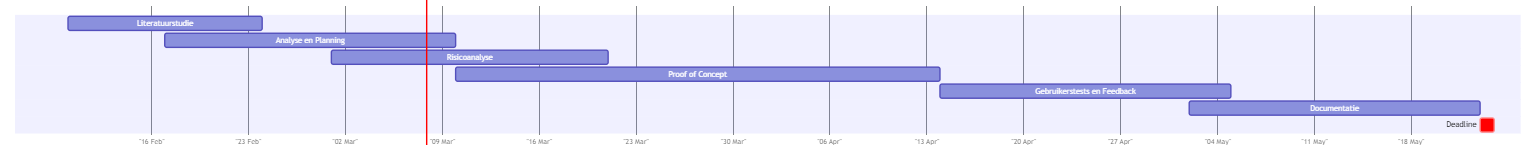
\includegraphics[scale=0.50]
  {img/ganttupdate.png}
  \caption{\label{fig:gantBP}Gantt-diagram van de onderzoeksplanning van 10 februari 2025 tot 23 mei 2025.}
\end{figure}
